\documentclass[11pt]{article}

\usepackage[margin=1in]{geometry}
\usepackage{amsmath,amssymb,amsthm}
\usepackage{booktabs}
\usepackage{enumitem}
\usepackage{graphicx}
\usepackage[most]{tcolorbox}
\usepackage{xurl}
\usepackage[hidelinks]{hyperref}

\setlength{\parindent}{0pt}
\setlength{\parskip}{0.45em}
\setlist{leftmargin=1.6em,itemsep=0.2em,topsep=0.2em}
\emergencystretch=2em

\newcommand{\rlvr}{\textsc{RLVR}}
\newcommand{\rl}{\textsc{RL}}
\newcommand{\llm}{\textsc{LLM}}
\newcommand{\vr}{\textsc{VR}}
\newcommand{\E}{\mathbb{E}}
\newcommand{\Var}{\mathrm{Var}}
\newcommand{\Cov}{\mathrm{Cov}}
\newcommand{\logit}{\mathrm{logit}}

\newtcolorbox{discussionbox}[1][]{
  colback=gray!5,
  colframe=black!35,
  title={Discussion},
  fonttitle=\bfseries,
  boxrule=0.5pt,
  arc=1mm,
  left=0.8em,
  right=0.8em,
  top=0.6em,
  bottom=0.6em,
  #1
}

\title{Verifiable Rewards as an Information Bottleneck}
\author{}
\date{\today}

\begin{document}

\maketitle

\begin{abstract}
Reinforcement learning with verifiable rewards has become a central recipe for improving reasoning and generation models because its feedback is cheap, objective, and nearly unbiased in domains with deterministic checkers. This paper studies the opposite side of this trade-off: verifiable rewards are reliable precisely because they compress rich trajectories into extremely low-bandwidth outcome signals. We formulate verifiable-reward learning as an information bottleneck, introduce metrics for dataset-level feedback budget, realized reward information, update strength, and information utilization, and analyze the resulting bottlenecks across AlphaZero-like self-play, \llm{} \rlvr{}, and diffusion-model \rlvr{}.
\end{abstract}

\section{Introduction}

Reinforcement learning with verifiable rewards (\rlvr{}) has become one of the most effective and scalable paradigms for improving reasoning models. In mathematical reasoning, code generation, theorem proving, games, and other domains with deterministic checkers, a trajectory can be evaluated by an external rule rather than by a learned reward model. This property gives verifiable rewards a distinctive advantage: they are cheap to obtain at scale, robust to subjective preference drift, and nearly unbiased with respect to the task outcome. Unlike learned reward models, which may introduce evaluator bias or create reward-hacking incentives, a verifier answers a much simpler question: did the final object satisfy the task specification?

This advantage, however, comes with a severe cost. Verifiable rewards trade reward bias for feedback bandwidth. A complex trajectory may contain many decisions, intermediate beliefs, partial discoveries, and local errors, but the verifier typically compresses all of them into a single terminal scalar, often a binary $0$--$1$ signal. The reward is not weak because it is wrong; it is weak because it is narrow. From the perspective of policy optimization, the verifier is a low-bandwidth feedback channel: it preserves the correctness of the final outcome while discarding most information about how that outcome was produced.

This low-bandwidth view helps explain several puzzling phenomena in recent \rlvr{} systems. When all rollouts for a prompt receive the same reward, group-relative methods obtain little or no useful advantage signal, even though the prompt may still contain learnable structure. When a reward is only observed at the end of a long reasoning trace, credit assignment becomes ambiguous: the update does not know whether success or failure came from search strategy, concept selection, arithmetic execution, formatting, or accidental exploration. As the policy becomes more confident, rollout diversity can collapse, reducing the number of distinct outcomes exposed to the verifier. Conversely, methods that seem algorithmically different--dense rewards, process supervision, entropy shaping, adaptive rollout allocation, self-verification, and trajectory-level exploration--can often be understood as attempts to recover, redistribute, or better use the limited information carried by verifiable feedback \cite{hybrid_reinforcement_2026,exploration_exploitation_rlvr_2026,lookahead_rollouts_2026,eepo_2026,no_prompt_left_behind_2026,igpo_2026}.

The bottleneck is especially sharp in \llm{} \rlvr{} on a fixed prompt dataset. In classical reinforcement learning, interacting with an environment can continually expose new states and new reward events. In contrast, with a fixed dataset and deterministic verifier, the source of verifier information is strongly bounded by the prompt set, rollout budget, and reward channel. Training does not create new ground-truth feedback; it changes which parts of a finite feedback budget are revealed by sampling, how that feedback is allocated across prompts, and how efficiently it is converted into policy updates. Thus many \rlvr{} algorithms should be evaluated not only by final accuracy, but also by how much verifier information they expose, how strong an update they produce from that information, and how much useful learning signal is wasted through zero-variance groups, redundant trajectories, or overly sparse rewards.

This paper studies verifiable-reward learning through this information-bottleneck lens. Our goal is not to argue that verifiable rewards should be replaced by learned rewards. Instead, we separate two issues that are often conflated: reward bias and reward information capacity. Verifiable rewards are attractive because they reduce bias; their limitation is that they provide a narrow channel through which task information reaches the optimizer. Understanding this trade-off allows us to compare AlphaZero-like self-play, \llm{} reasoning, and diffusion generation under a common vocabulary.

We make the following contributions:
\begin{enumerate}
  \item We formulate verifiable-reward learning as a low-bandwidth feedback channel, making explicit the distinction between reward bias and reward information capacity.
  \item We introduce quantitative notions for dataset-level feedback budget, realized reward information, update strength, and information utilization. In particular, we emphasize that for \llm{} \rlvr{} on a fixed dataset with deterministic verifiers, the available verifier information is bounded and often effectively fixed by the dataset, rollout budget, and reward channel.
  \item We analyze the information bottleneck across three settings: AlphaZero-like self-play in board-game-style environments, \llm{} \rlvr{}, and diffusion-model \rlvr{}. Across these domains, we identify different ways to improve information efficiency, including richer rollout diversity, adaptive allocation of verifier queries, dense or trajectory-level feedback, and reward-aware credit assignment.
\end{enumerate}

By viewing verifiable rewards as an information bottleneck, we obtain a unified explanation for why sparse outcome feedback can be reliable yet inefficient, why some prompts contribute little to learning despite being meaningful, and why recent algorithmic improvements often work by increasing the effective bandwidth between the verifier and the policy optimizer.

\section{Related Work}

\paragraph{RL for LLM reasoning and verifiable rewards.}
Reinforcement learning has become a central post-training tool for improving mathematical reasoning, code generation, and other tasks where outcomes can be checked automatically. Systems such as DAPO scale reinforcement learning for \llm{} reasoning with mechanisms aimed at stable optimization and entropy control \cite{dapo_2025}. Recent \rlvr{} work studies why verifier-based training can improve reasoning, how spurious or clipped rewards interact with entropy, and how exploration changes the effectiveness of group-relative updates \cite{exploration_exploitation_rlvr_2026,wen2025reinforcement,he2025random}. Our work is complementary: rather than proposing a new optimizer, we formulate verifier feedback as a low-bandwidth information channel and measure its usable signal through reward variance and reward--score covariance.

\paragraph{Entropy, exploration, and zero-variance prompts.}
Several recent methods identify entropy collapse, insufficient rollout diversity, or zero-variance prompt groups as bottlenecks in \llm{} \rlvr{}. DAPO emphasizes entropy-stabilized large-scale RL, while follow-up work studies selective entropy regularization, bidirectional entropy modulation, entropy-curve control, and quantile-based advantage estimation \cite{dapo_2025,siren2025,asymgrpo2026,entrocraft2026,qae2025}. Other methods increase trajectory-level diversity or explicitly handle zero-variance prompts \cite{lookahead_rollouts_2026,eepo_2026,no_prompt_left_behind_2026}. These methods can be viewed through our lens as attempts to increase exposed verifier variance, keep prompts near the decision boundary, or improve the conversion from reward variation to policy updates.

\paragraph{Sparse, dense, and hybrid rewards.}
Verifiable rewards are attractive because they are low-bias with respect to precise task specifications, but they often compress rich trajectories into terminal binary outcomes. Hybrid and dense-reward methods attempt to recover part of the missing feedback bandwidth by combining sparse verifiers with learned reward models or graded supervisory signals \cite{hybrid_reinforcement_2026}. Our formulation separates this issue into reward-model bias, evaluator noise, reward variance, and update alignment. This distinction is important because denser feedback is useful only when it adds policy-controllable, update-aligned variance rather than merely increasing noisy reward dispersion.

\paragraph{Self-play and renewable feedback.}
AlphaZero-like self-play demonstrates a different way to overcome sparse terminal rewards: the reward itself may remain binary and terminal, but the rollout distribution is renewed by playing against an opponent of comparable strength \cite{silver2017mastering}. This keeps outcomes near a high-variance frontier and makes the reward-information integral grow with continued self-play. We use this regime as a contrast to fixed-dataset \llm{} \rlvr{}, where the prompt-verifier source is fixed and many prompts eventually become all-correct or all-wrong.

\paragraph{Diffusion and generative-model RL.}
Diffusion models introduce long generation trajectories and delayed or multi-objective feedback \cite{ho2020denoising}. In this setting, the main bottleneck is not only whether final-sample rewards have variance, but also whether those rewards have useful covariance with intermediate denoising decisions. The diffusion section of this paper is currently left as a placeholder, but the common covariance formulation is designed to extend to image and video generation rewards, including aesthetics, prompt alignment, temporal consistency, and safety.

\section{Problem Formulation}

This section defines the objects used throughout the paper and introduces two quantities that will be used to analyze reward-model-driven learning: local update strength and global reward-information mass. The key object is not a reward attached directly to a state, but a reward obtained by first sampling rollouts from the current model and then evaluating those rollouts with a reward model.

\subsection{Models, Rollouts, and Rewards}

A standard reinforcement learning problem can be written as a Markov decision process
\[
  \mathcal{M}=(\mathcal{S},\mathcal{A},P,\rho_0,\gamma),
\]
where $\mathcal{S}$ is the state space, $\mathcal{A}$ is the action space, $P(s'\mid s,a)$ is the environment transition model, $\rho_0$ is the initial-state distribution, and $\gamma$ is the discount factor. A policy $\pi_\theta(a\mid s)$, together with the environment dynamics, induces a rollout distribution
\[
  \tau \sim q_\theta(\cdot),
  \qquad
  \tau=(s_0,a_0,s_1,a_1,\ldots).
\]
A reward model then maps the sampled rollout to a scalar reward,
\[
  R = \mathsf{R}_\psi(\tau).
\]
In classical \rl{}, $\mathsf{R}_\psi$ may simply be the hand-designed return functional
\[
  \mathsf{R}_\psi(\tau)=G(\tau)=\sum_{t\ge 0}\gamma^t r(s_t,a_t,s_{t+1}).
\]
In learned-reward settings, $\mathsf{R}_\psi$ may be a trained reward model. In verifiable-reward settings, $\mathsf{R}_\psi$ is a deterministic or nearly deterministic verifier.

For \llm{} and diffusion-model \rlvr{}, we use the conditional version of the same setup. A task or prompt $x\sim \mathcal{D}$ is the initial condition, the rollout model induces a trajectory distribution
\[
  \tau \sim q_\theta(\cdot\mid x),
\]
and the reward model evaluates the sampled trajectory:
\[
  R=\mathsf{R}_\psi(x,\tau).
\]
Here $\tau$ may be a reasoning trace, a program-generation trajectory, a game trajectory, an image-generation trajectory, or a denoising path. A binary verifier is the special case
\[
  \mathsf{R}_\psi(x,\tau)=V(x,\tau)\in\{0,1\}.
\]
Thus the reward is a random variable because the rollout is sampled from the current model distribution, even when the reward model itself is deterministic.

The conditional objective is
\[
  J(\theta)
  =
  \E_{x\sim \mathcal{D}}
  \E_{\tau\sim q_\theta(\cdot\mid x)}
  \left[
    \mathsf{R}_\psi(x,\tau)
  \right].
\]
Optional regularizers such as KL penalties to a reference model can be added to this objective, but the central question studied here concerns the information carried by the reward signal produced by $\mathsf{R}_\psi$ under the rollout distribution $q_\theta$.

\subsection{Local Update Strength}

Fix a prompt or initial condition $x$. Let
\[
  s_\theta(x,\tau)=\nabla_\theta \log q_\theta(\tau\mid x)
\]
be the score vector of the sampled rollout. In autoregressive \llm{} policies, this score decomposes into token log-probability gradients. In classical \rl{}, environment transitions independent of $\theta$ vanish from the score, leaving the usual sum of action log-probability gradients. In diffusion or flow models, $s_\theta$ is the score of the sampled denoising or generation trajectory.

The prompt-level policy-gradient contribution is
\[
  g_\theta(x)
  =
  \nabla_\theta
  \E_{\tau\sim q_\theta(\cdot\mid x)}
  [\mathsf{R}_\psi(x,\tau)].
\]
Using the score-function identity,
\[
  g_\theta(x)
  =
  \E_{\tau\sim q_\theta(\cdot\mid x)}
  \left[
    \mathsf{R}_\psi(x,\tau)s_\theta(x,\tau)
  \right].
\]
Since $\E_{\tau\sim q_\theta(\cdot\mid x)}[s_\theta(x,\tau)]=0$ under the usual support assumptions, this can be written as a covariance:
\[
  g_\theta(x)
  =
  \Cov_{\tau\sim q_\theta(\cdot\mid x)}
  \left(
    \mathsf{R}_\psi(x,\tau),\,
    s_\theta(x,\tau)
  \right).
\]
Thus the local update is strong only when reward variation across rollouts aligns with directions in model probability space. A reward model can be unbiased or even exactly verifiable, but if all rollouts around $x$ receive the same reward, this local covariance vanishes.

We define the local update strength as
\[
  \mathcal{U}_\theta(x)=\|g_\theta(x)\|_2^2.
\]
This quantity separates two factors: the reward-side variation exposed by rollout sampling and the policy-side sensitivity of those sampled rollouts. By Cauchy--Schwarz,
\[
  \mathcal{U}_\theta(x)
  \le
  \Var_{\tau\sim q_\theta(\cdot\mid x)}
  [\mathsf{R}_\psi(x,\tau)]
  \cdot
  \E_{\tau\sim q_\theta(\cdot\mid x)}
  \left[
    \left\|s_\theta(x,\tau)\right\|_2^2
  \right].
\]
The reward variance under the rollout model is therefore an upper-level proxy for whether a prompt can produce a nontrivial policy update at all. For a binary verifier, if
\[
  p_\theta(x)=\Pr_{\tau\sim q_\theta(\cdot\mid x)}[V(x,\tau)=1],
\]
then
\[
  \Var[V(x,\tau)\mid x]=p_\theta(x)(1-p_\theta(x)).
\]
This term is zero when the rollout model is always wrong or always correct on $x$, and maximal when $p_\theta(x)=1/2$.

We will use the following shorthand for this local reward-side signal:
\[
  \mathcal{V}_\theta(x)
  =
  \Var_{\tau\sim q_\theta(\cdot\mid x)}
  \big[\mathsf{R}_\psi(x,\tau)\big].
\]
This is the local variance of reward-model outputs under the current rollout distribution. Its accumulation over training will define the global reward-information mass below.

This covariance view also gives a compact interpretation of group-relative policy optimization. For a prompt $x$, sample a group $\{\tau_j\}_{j=1}^K$ from the rollout model and write
\[
  r_j=\mathsf{R}_\psi(x,\tau_j),\qquad
  s_j=s_\theta(x,\tau_j),\qquad
  \bar r=\frac{1}{K}\sum_{j=1}^K r_j.
\]
Ignoring clipping, KL regularization, and reward-standard-deviation normalization, the group-centered policy-gradient estimator is
\[
  \widehat g_{\mathrm{GRPO}}(x)
  =
  \frac{1}{K}\sum_{j=1}^K (r_j-\bar r)s_j.
\]
Since $\sum_j(r_j-\bar r)=0$, this is exactly the empirical covariance between reward-model outputs and rollout scores:
\[
  \widehat g_{\mathrm{GRPO}}(x)
  =
  \frac{1}{K}\sum_{j=1}^K
  (r_j-\bar r)(s_j-\bar s)
  =
  \widehat{\Cov}_{K}(r,s\mid x),
  \qquad
  \bar s=\frac{1}{K}\sum_{j=1}^K s_j.
\]
With reward normalization, the same covariance direction is rescaled by the empirical reward standard deviation. With clipping and KL penalties, this covariance update is further constrained by the trust-region-like optimization geometry. The basic point remains: in group-relative \rlvr{}, useful local learning signal is the covariance between reward-model evaluations and model-score directions over sampled rollouts.

\subsection{Global Reward-Information Mass}

Local update strength describes whether one prompt can produce an update at a particular policy. We also need a global quantity that tracks how much reward-side learning signal is exposed over the entire training run.

Let $\theta(t)$ denote the rollout model along a continuous-time training trajectory, let $\alpha(t)$ denote the learning rate (or update-size schedule), and let $T_{\mathrm{train}}$ be the end of training. We define the global reward-information mass as the learning-rate-weighted integral of local reward variance from the beginning to the end of training:
\[
  \mathcal{I}_{\mathrm{train}}
  =
  \int_0^{T_{\mathrm{train}}}
  \alpha(t)\,
  \E_{x\sim \mathcal{D}}
  \left[
    \Var_{\tau\sim q_{\theta(t)}(\cdot\mid x)}
    \big[
      \mathsf{R}_\psi(x,\tau)
    \big]
  \right]
  dt.
\]
Equivalently, using the shorthand above,
\[
  \mathcal{I}_{\mathrm{train}}
  =
  \int_0^{T_{\mathrm{train}}}
  \alpha(t)\,
  \E_{x\sim \mathcal{D}}
  \left[
    \mathcal{V}_{\theta(t)}(x)
  \right]
  dt.
\]
For a finite prompt dataset $\mathcal{D}=\{x_i\}_{i=1}^N$ and a binary verifier, this becomes
\[
  \mathcal{I}_{\mathrm{train}}
  =
  \int_0^{T_{\mathrm{train}}}
  \alpha(t)\,
  \frac{1}{N}\sum_{i=1}^N
  p_t(x_i)(1-p_t(x_i))
  dt,
  \qquad
  p_t(x_i)=\Pr_{\tau\sim q_{\theta(t)}(\cdot\mid x_i)}[V(x_i,\tau)=1].
\]
In discrete training with batches $\mathcal{B}_t$, this quantity is estimated by
\[
  \widehat{\mathcal{I}}_{0:T}
  =
  \sum_{t=0}^{T-1}
  \alpha_t\,
  \frac{1}{|\mathcal{B}_t|}
  \sum_{x_i\in \mathcal{B}_t}
  \widehat{\Var}\left(
    r_{i,1},\ldots,r_{i,K}
  \right),
\]
where $r_{i,j}=\mathsf{R}_\psi(x_i,\tau_{i,j})$ is the reward-model output for the $j$-th rollout of prompt $x_i$.

This definition is not meant to be a full Shannon mutual information between the reward model and the parameters. Rather, it is an optimization-facing measure of reward-side information that can be converted into policy updates. It intentionally weights local reward dispersion by the update size: reward variance observed when the optimizer takes no step contributes little to learning, while variance observed under a larger update budget contributes more.

\begin{discussionbox}[title={Discussion: Why variance rather than entropy?}]
One could instead measure the entropy of reward-model outputs, e.g. $H(\mathsf{R}_\psi(x,\tau))$. We use variance because the quantity is meant to describe optimization-relevant signal, not only uncertainty of the reward symbol. Entropy loses reward scale: replacing a scalar reward $R$ by $cR$ leaves the discrete outcome entropy unchanged whenever the support labels are unchanged, but it scales the policy-gradient covariance and the update magnitude by $c$. Variance is shift-invariant and scale-sensitive, matching the fact that policy-gradient updates depend on reward differences. For binary rewards, both $H(\mathrm{Bernoulli}(p))$ and $p(1-p)$ vanish at $p\in\{0,1\}$ and peak at $p=1/2$, but variance extends naturally to scalar or dense rewards where the numerical gaps between rollout outcomes directly affect learning strength. Thus $\int \alpha(t)\E_x[\Var_{\tau\sim q_{\theta(t)}}(\mathsf{R}_\psi(x,\tau)\mid x)]dt$ should be read as reward-variance mass, an optimizer-facing proxy for usable reward-model information.
\end{discussionbox}

The definition also makes explicit why fixed-dataset \llm{} \rlvr{} is different from open-ended environment interaction. With deterministic verifiers and a fixed prompt set, the reward model is fixed; training changes $q_{\theta(t)}(\tau\mid x)$ and therefore changes which rewards are exposed, but it does not create new ground-truth reward labels outside the dataset-verifier system. For binary rewards,
\[
  0
  \le
  \mathcal{I}_{\mathrm{train}}
  \le
  \frac{1}{4}\int_0^{T_{\mathrm{train}}} \alpha(t)\,dt.
\]
Thus the central algorithmic question is how to expose and convert this bounded reward-information mass efficiently. Rollout diversification can move prompts away from zero-variance regions, adaptive allocation can spend reward-model queries where $p_t(x)(1-p_t(x))$ is high, and dense or trajectory-level rewards can replace a low-bandwidth terminal signal with higher-bandwidth intermediate feedback.

\section{Reward-Model Bias, Variance, and Multi-Objective Feedback}

The previous section defined reward-information mass from the variance of reward-model outputs under the rollout distribution. This section separates three related but distinct issues: whether the reward model is biased, whether its evaluations are noisy, and whether the task is better described by multiple reward channels rather than a single scalar.

\subsection{Bias and Evaluator Variance}

Let $U^\star(x,\tau)$ denote the target utility that we would like the policy to optimize. This may be final correctness, human preference, game outcome, visual quality, safety, or any task-specific objective. A reward model $\mathsf{R}_\psi$ is an evaluator of the sampled rollout. If the evaluator is stochastic, we write
\[
  R \sim \mathsf{R}_\psi(\cdot\mid x,\tau),
  \qquad
  \mu_\psi(x,\tau)=\E[R\mid x,\tau].
\]
The reward-model bias and evaluator variance are
\[
  b_\psi(x,\tau)=\mu_\psi(x,\tau)-U^\star(x,\tau),
  \qquad
  \sigma_\psi^2(x,\tau)=\Var[R\mid x,\tau].
\]
A deterministic verifier is the special case where $\sigma_\psi^2(x,\tau)=0$. When the verifier exactly matches the task specification, its bias with respect to the specified outcome is also zero. This is the main appeal of verifiable rewards: they can be low-bias and low-noise evaluators.

However, low evaluator bias is different from high training signal. Under the rollout distribution, the reward random variable has the decomposition
\[
  \Var_{\tau\sim q_\theta,\,R\sim \mathsf{R}_\psi}
  [R\mid x]
  =
  \Var_{\tau\sim q_\theta}
  [\mu_\psi(x,\tau)\mid x]
  +
  \E_{\tau\sim q_\theta}
  [\sigma_\psi^2(x,\tau)\mid x].
\]
The first term is rollout-induced reward variation: it reflects whether different sampled trajectories receive different expected evaluations. The second term is evaluator noise: it can increase observed reward variance without necessarily adding useful directional signal. Thus a high-variance reward channel is not automatically informative; the variance must align with policy-controllable differences among rollouts.

\subsection{Bias of the Policy Update}

The reward-model gradient induced by the evaluator mean is
\[
  g_\psi(x)
  =
  \Cov_{\tau\sim q_\theta(\cdot\mid x)}
  \left(
    \mu_\psi(x,\tau),
    s_\theta(x,\tau)
  \right),
  \qquad
  s_\theta(x,\tau)=\nabla_\theta \log q_\theta(\tau\mid x).
\]
The ideal gradient for the target utility is
\[
  g^\star(x)
  =
  \Cov_{\tau\sim q_\theta(\cdot\mid x)}
  \left(
    U^\star(x,\tau),
    s_\theta(x,\tau)
  \right).
\]
Their difference is
\[
  g_\psi(x)-g^\star(x)
  =
  \Cov_{\tau\sim q_\theta(\cdot\mid x)}
  \left(
    b_\psi(x,\tau),
    s_\theta(x,\tau)
  \right).
\]
Therefore reward-model bias matters only through its covariance with controllable rollout directions. A biased reward model is especially harmful when its bias is systematically aligned with high-probability policy changes. Conversely, a reward model may contain pointwise bias that is less damaging if the bias is nearly constant over the rollouts reachable by the current policy, because constant offsets do not affect policy-gradient covariance.

This motivates an update-alignment measure:
\[
  \mathrm{Align}_\theta(x)
  =
  \frac{
    \langle g_\psi(x),g^\star(x)\rangle
  }{
    \|g_\psi(x)\|_2\|g^\star(x)\|_2+\epsilon
  }.
\]
The reward-information mass from Section~2 measures how much reward-side variation is exposed, while update alignment measures whether that variation points in the desired direction.

\subsection{Variance of the Gradient Estimator}

For a group of $K$ sampled rollouts, a generic centered estimator has the form
\[
  \widehat g(x)
  =
  \frac{1}{K}\sum_{j=1}^K
  (R_j-\bar R)s_j.
\]
Its estimator variance depends not only on rollout diversity, but also on evaluator noise. If the evaluator noise is conditionally independent given $(x,\tau)$, then the second-moment contribution contains the term
\[
  \E_{\tau\sim q_\theta(\cdot\mid x)}
  \left[
    \sigma_\psi^2(x,\tau)
    s_\theta(x,\tau)s_\theta(x,\tau)^\top
  \right].
\]
This term increases gradient-estimator variance without changing the expected update direction. Thus the usual bias--variance trade-off for reward models should be refined into a three-way trade-off:
\[
  \text{reward bias}
  \quad
  \text{vs.}
  \quad
  \text{evaluator noise}
  \quad
  \text{vs.}
  \quad
  \text{feedback bandwidth}.
\]

\begin{discussionbox}[title={Discussion: Verifiers and learned reward models}]
Verifiable rewards occupy one corner of this trade-off. They are often low-bias and low-noise with respect to a precise task specification, but they may have extremely low feedback bandwidth, especially when they return only a terminal binary outcome. Learned reward models can provide dense scalar feedback and increase rollout-induced reward variance, but they may introduce bias, evaluator noise, and reward hacking. From this perspective, the question is not whether verifiers or reward models are universally better. The question is how much usable update signal each evaluator provides per unit of bias and noise.
\end{discussionbox}

\subsection{Two Sources of Multiple Rewards}

Multiple rewards arise in two different ways. First, the same task may be evaluated by several reward models. Second, a training dataset may contain different tasks, each with its own reward. Both cases turn policy optimization into a scalarization of multiple objectives, but they have different sources of variance and conflict.

\paragraph{Same task, different rewards.}
For a fixed task $x$, one rollout may be evaluated by several reward channels. A reasoning model may need correctness, brevity, safety, and format compliance. A diffusion model may need aesthetics, prompt alignment, object count, identity preservation, physical consistency, and safety. We write this form as
\[
  \mathbf{R}_\psi(x,\tau)
  =
  \left(
    R_\psi^{(1)}(x,\tau),\ldots,R_\psi^{(m)}(x,\tau)
  \right)^\top
  \in \mathbb{R}^m.
\]
Given a scalarization weight vector $w\in\mathbb{R}^m$, the scalar reward is
\[
  R_w(x,\tau)=w^\top \mathbf{R}_\psi(x,\tau).
\]
The local reward variance under this scalarization is
\[
  \mathcal{V}_\theta^w(x)
  =
  \Var_{\tau\sim q_\theta(\cdot\mid x)}
  [w^\top \mathbf{R}_\psi(x,\tau)]
  =
  w^\top
  \Sigma_\theta^R(x)
  w,
\]
where
\[
  \Sigma_\theta^R(x)
  =
  \Cov_{\tau\sim q_\theta(\cdot\mid x)}
  \left(
    \mathbf{R}_\psi(x,\tau)
  \right)
\]
is the reward covariance matrix across sampled rollouts.

The scalarized global reward-information mass is therefore
\[
  \mathcal{I}_{\mathrm{train}}^w
  =
  \int_0^{T_{\mathrm{train}}}
  \alpha(t)
  \E_{x\sim\mathcal{D}}
  \left[
    w^\top \Sigma_{\theta(t)}^R(x)w
  \right]
  dt.
\]
If the scalarization is not fixed in advance, the more primitive object is the matrix-valued reward-information mass
\[
  \mathbf{I}_{\mathrm{train}}^{R}
  =
  \int_0^{T_{\mathrm{train}}}
  \alpha(t)
  \E_{x\sim\mathcal{D}}
  \left[
    \Sigma_{\theta(t)}^R(x)
  \right]
  dt.
\]
This matrix records how much reward variation is available along each objective and how much the objectives co-vary over sampled rollouts. Its trace measures total marginal reward variance, while its spectrum reveals whether the reward signal is concentrated in a few redundant directions or spread across many independent objectives.

Multi-objective feedback also has an update-space view. Define
\[
  G_\theta(x)
  =
  \Cov_{\tau\sim q_\theta(\cdot\mid x)}
  \left(
    \mathbf{R}_\psi(x,\tau),
    s_\theta(x,\tau)
  \right)
  \in \mathbb{R}^{m\times d},
\]
whose $k$-th row is the policy-gradient direction induced by objective $k$. For scalarization $w$, the update is
\[
  g_w(x)=G_\theta(x)^\top w.
\]
Objective conflict can be studied through the update Gram matrix
\[
  C_\theta(x)=G_\theta(x)G_\theta(x)^\top,
\]
where $C_{\theta,ij}(x)=\langle g_i(x),g_j(x)\rangle$ measures whether objectives $i$ and $j$ push the policy in compatible or competing directions. This distinguishes two cases that scalar reward variance alone cannot separate: multiple objectives may provide independent information but still agree in update space, or they may expose rich information while inducing conflicting policy updates.

\paragraph{Different tasks, different rewards.}
A second source of multiple rewards is the dataset itself. Suppose a dataset is a mixture of tasks,
\[
  \mathcal{D}=\sum_{k=1}^m \rho_k \mathcal{D}_k,
  \qquad
  \sum_{k=1}^m \rho_k=1,
\]
where task family $k$ has reward model $\mathsf{R}_{\psi_k}^{(k)}$. The training objective is a scalarized multi-task objective:
\[
  J(\theta)
  =
  \sum_{k=1}^m \rho_k
  \E_{x\sim \mathcal{D}_k}
  \E_{\tau\sim q_\theta(\cdot\mid x)}
  \left[
    \mathsf{R}_{\psi_k}^{(k)}(x,\tau)
  \right].
\]
The task-level gradient is
\[
  g_k(\theta)
  =
  \E_{x\sim \mathcal{D}_k}
  \Cov_{\tau\sim q_\theta(\cdot\mid x)}
  \left(
    \mathsf{R}_{\psi_k}^{(k)}(x,\tau),
    s_\theta(x,\tau)
  \right),
\]
and the dataset update is the weighted sum
\[
  g_{\mathcal{D}}(\theta)=\sum_{k=1}^m \rho_k g_k(\theta).
\]
This is the sense in which \llm{} \rlvr{} on a dataset is often multi-objective: even if every prompt has only one binary verifier, different prompts or task families define different local objectives whose gradients may agree, interfere, or dominate one another.

The same reward-information view applies at the task level:
\[
  \mathcal{I}_{\mathrm{train}}^{(k)}
  =
  \int_0^{T_{\mathrm{train}}}
  \alpha(t)\,
  \E_{x\sim\mathcal{D}_k}
  \left[
    \Var_{\tau\sim q_{\theta(t)}(\cdot\mid x)}
    \big[
      \mathsf{R}_{\psi_k}^{(k)}(x,\tau)
    \big]
  \right]
  dt.
\]
The scalar dataset-level mass is $\sum_k \rho_k \mathcal{I}_{\mathrm{train}}^{(k)}$, but this scalar can hide imbalance: a small subset of tasks may dominate the reward variance and update strength, while other tasks consume rollouts but produce near-zero local signal.

For a finite dataset $\mathcal{D}=\{x_i\}_{i=1}^N$, it is often useful to work with the unnormalized total information budget rather than the dataset average. Define the per-example reward-information mass as
\[
  \mathcal{I}_i
  =
  \int_0^{T_{\mathrm{train}}}
  \alpha(t)\,
  \Var_{\tau\sim q_{\theta(t)}(\cdot\mid x_i)}
  \left[
    \mathsf{R}_{\psi_i}^{(i)}(x_i,\tau)
  \right]
  dt,
\]
where $\mathsf{R}_{\psi_i}^{(i)}$ denotes the reward model or verifier associated with example $x_i$. The dataset total reward-information mass is
\[
  \mathcal{I}_{\mathcal{D}}^{\mathrm{tot}}
  =
  \sum_{i=1}^N \mathcal{I}_i.
\]
If every example has per-example mass bounded by $I_{\max}$, then
\[
  \mathcal{I}_{\mathcal{D}}^{\mathrm{tot}}
  \le
  N I_{\max}.
\]
For binary rewards, a crude universal bound is
\[
  \mathcal{I}_i
  \le
  \frac{1}{4}
  \int_0^{T_{\mathrm{train}}}
  \alpha(t)\,dt,
  \qquad
  \mathcal{I}_{\mathcal{D}}^{\mathrm{tot}}
  \le
  \frac{N}{4}
  \int_0^{T_{\mathrm{train}}}
  \alpha(t)\,dt.
\]
This scaling makes explicit that fixed-dataset \llm{} \rlvr{} has a finite verifier-information budget that grows at most linearly with the number of examples, before accounting for redundancy and gradient conflict across tasks.

\begin{discussionbox}[title={Claim to prove: subadditivity across task sets}]
The total dataset mass above is an additive bookkeeping quantity. For usable information, however, two task sets trained through a shared rollout model and shared parameter updates may not preserve all information available from each set in isolation. In the terminology of this paper, we will formalize this cross-task interference as a subadditivity statement, e.g.
\[
  \mathcal{I}_{A\cup B}^{\mathrm{usable}}
  \le
  \mathcal{I}_{A}^{\mathrm{usable}}
  +
  \mathcal{I}_{B}^{\mathrm{usable}}.
\]
Strict inequality may arise from redundant reward variance, shared rollout budget, finite update bandwidth, and conflicting task gradients. This is the dataset-level sense in which the union of tasks may contain less usable reward information than the sum of separately measured task information.
\end{discussionbox}

\begin{discussionbox}[title={Discussion: Dataset RL as multi-objective RL}]
In fixed-dataset \llm{} \rlvr{}, it is useful to view each prompt, benchmark, or task family as an objective. The usual dataset average is a scalarization chosen by the data mixture. This scalarization may look innocuous, but it determines which reward signals dominate training. Easy prompts can have low variance because all rollouts are correct; impossible prompts can have low variance because all rollouts are wrong; medium-difficulty prompts can dominate the effective update. Thus the multi-objective problem is not only about different reward heads, but also about how a dataset allocates update bandwidth across many local objectives.
\end{discussionbox}

In the rest of the paper, this bias--variance--multi-objective view will be used to compare three regimes. Traditional games often have low-bias outcome rewards but can generate new rollouts through environment interaction. \llm{} \rlvr{} often has a fixed prompt-verifier source, so the main issue is exposing and converting a bounded reward-variance budget. Diffusion \rlvr{} often has long generation trajectories and naturally multi-objective reward models, so its main issue is assigning dense, low-bias, multi-objective feedback to intermediate denoising decisions.

\section{AlphaZero-like Self-Play: A Renewable Verifiable Reward Source}

We now specialize the traditional \rl{} comparison to AlphaZero-like self-play in board games. This is the cleanest contrast to fixed-dataset \llm{} \rlvr{}: both settings may use terminal, sparse, verifiable rewards, but AlphaZero-like training continually generates new games against a policy of comparable strength. As a result, the terminal reward distribution can remain high-variance throughout training, rather than collapsing as the model solves or fails a fixed set of prompts.

\subsection{Self-Play Keeps the Outcome Near the Decision Boundary}

Consider a two-player zero-sum game. At training time $t$, an AlphaZero-like agent uses the current policy/value model, often combined with Monte Carlo tree search, to generate self-play games. A trajectory
\[
  \tau \sim q_{\theta(t),\theta(t)}(\cdot)
\]
is produced by matching the current agent against itself. The terminal reward from one player's perspective is
\[
  z(\tau)\in\{0,1\},
\]
where $1$ denotes a win and $0$ denotes a loss. Draws can be ignored, folded into a half reward, or handled as a third outcome; the binary case makes the information argument most transparent.

The local reward-side signal is
\[
  \mathcal{V}_{\theta(t)}^{\mathrm{sp}}
  =
  \Var_{\tau\sim q_{\theta(t),\theta(t)}}[z(\tau)]
  =
  p_t(1-p_t),
\]
where
\[
  p_t=\Pr_{\tau\sim q_{\theta(t),\theta(t)}}[z(\tau)=1].
\]
Because the two players are copies of the same learning system, self-play tends to keep the matchup balanced. Up to first-move advantage, stochasticity, search noise, and draw handling, one should expect
\[
  p_t \approx \frac{1}{2},
  \qquad
  \mathcal{V}_{\theta(t)}^{\mathrm{sp}}
  \approx
  \frac{1}{4}.
\]
Thus the reward distribution remains approximately ``half zero, half one.'' Unlike a fixed prompt whose verifier outcomes may become all-correct or all-wrong, a self-play game does not become trivial merely because the agent improves: its opponent improves with it.

\subsection{The Information Integral Need Not Saturate}

Using the global reward-information definition from Section~2, the self-play reward-information mass is
\[
  \mathcal{I}_{\mathrm{sp}}(T)
  =
  \int_0^T
  \alpha(t)
  \Var_{\tau\sim q_{\theta(t),\theta(t)}}[z(\tau)]
  dt.
\]
If self-play keeps the terminal outcome non-degenerate, i.e. there exists a constant $c>0$ such that
\[
  \Var_{\tau\sim q_{\theta(t),\theta(t)}}[z(\tau)]\ge c
  \quad
  \text{for most }t,
\]
then
\[
  \mathcal{I}_{\mathrm{sp}}(T)
  \ge
  c\int_0^T \alpha(t)\,dt.
\]
Therefore, whenever the cumulative update budget $\int_0^T\alpha(t)dt$ grows without bound, the self-play information integral is also unbounded. Even for finite training, the key point is that the information budget is controlled by the number of generated self-play games and the cumulative update mass, not by a fixed dataset size.

This is the fundamental difference from fixed-dataset \llm{} \rlvr{}. For a fixed prompt set with deterministic binary verifiers, each prompt has a bounded reward-variance mass and the dataset total is bounded by a quantity scaling with $N$. In AlphaZero-like self-play, there is no fixed list of questions whose outcomes are gradually exhausted. The learner keeps producing fresh games against its current level, and the terminal reward remains a renewable source of high-variance feedback.

\subsection{Why Improvement Does Not Collapse Reward Variance}

The apparent paradox is that the agent becomes stronger, yet its win-rate in self-play does not approach one. The reason is that self-play measures the current policy against a moving reference. Let $\pi_{\theta(t)}$ be the current policy and suppose both sides use the same or closely related policy. Then absolute playing strength can improve while the self-play win probability remains close to balanced:
\[
  \Pr(\pi_{\theta(t)} \text{ beats } \pi_{\theta(t)}) \approx \frac{1}{2}.
\]
This makes self-play an automatic curriculum. The task distribution tracks the learner's ability: when the model improves, the opponent and generated positions improve as well. The verifier still gives only a terminal outcome, but the rollout distribution continually refreshes the set of contested decisions that can affect the outcome.

From the covariance view, this means AlphaZero-like training attempts to maintain nonzero covariance between terminal outcome and policy-score directions:
\[
  g_{\mathrm{sp}}(\theta)
  =
  \Cov_{\tau\sim q_{\theta,\theta}}
  \left(
    z(\tau),
    \nabla_\theta \log q_\theta(\tau)
  \right).
\]
The terminal reward is sparse, but it is repeatedly queried at the frontier of the current policy's competence. This is exactly the regime where $p(1-p)$ is large.

\subsection{Connect Four Evidence}

We tested this distinction in two rounds of Connect Four experiments. The results support the view that AlphaZero-like self-play is fundamentally different from fixed-dataset \rlvr{}. With a fixed prompt or verifier source, improvement eventually pushes many examples into all-correct or all-wrong regimes, where the binary verifier carries little local contrast. In self-play, by contrast, the opponent and the position distribution co-evolve with the current policy. The training data therefore keeps moving toward the model's competence boundary. Even though the reward remains only a terminal $0/1$ outcome, self-play can sustain substantial outcome variance and act as a renewable source of verifier feedback.

\begin{figure}[t]
  \centering
  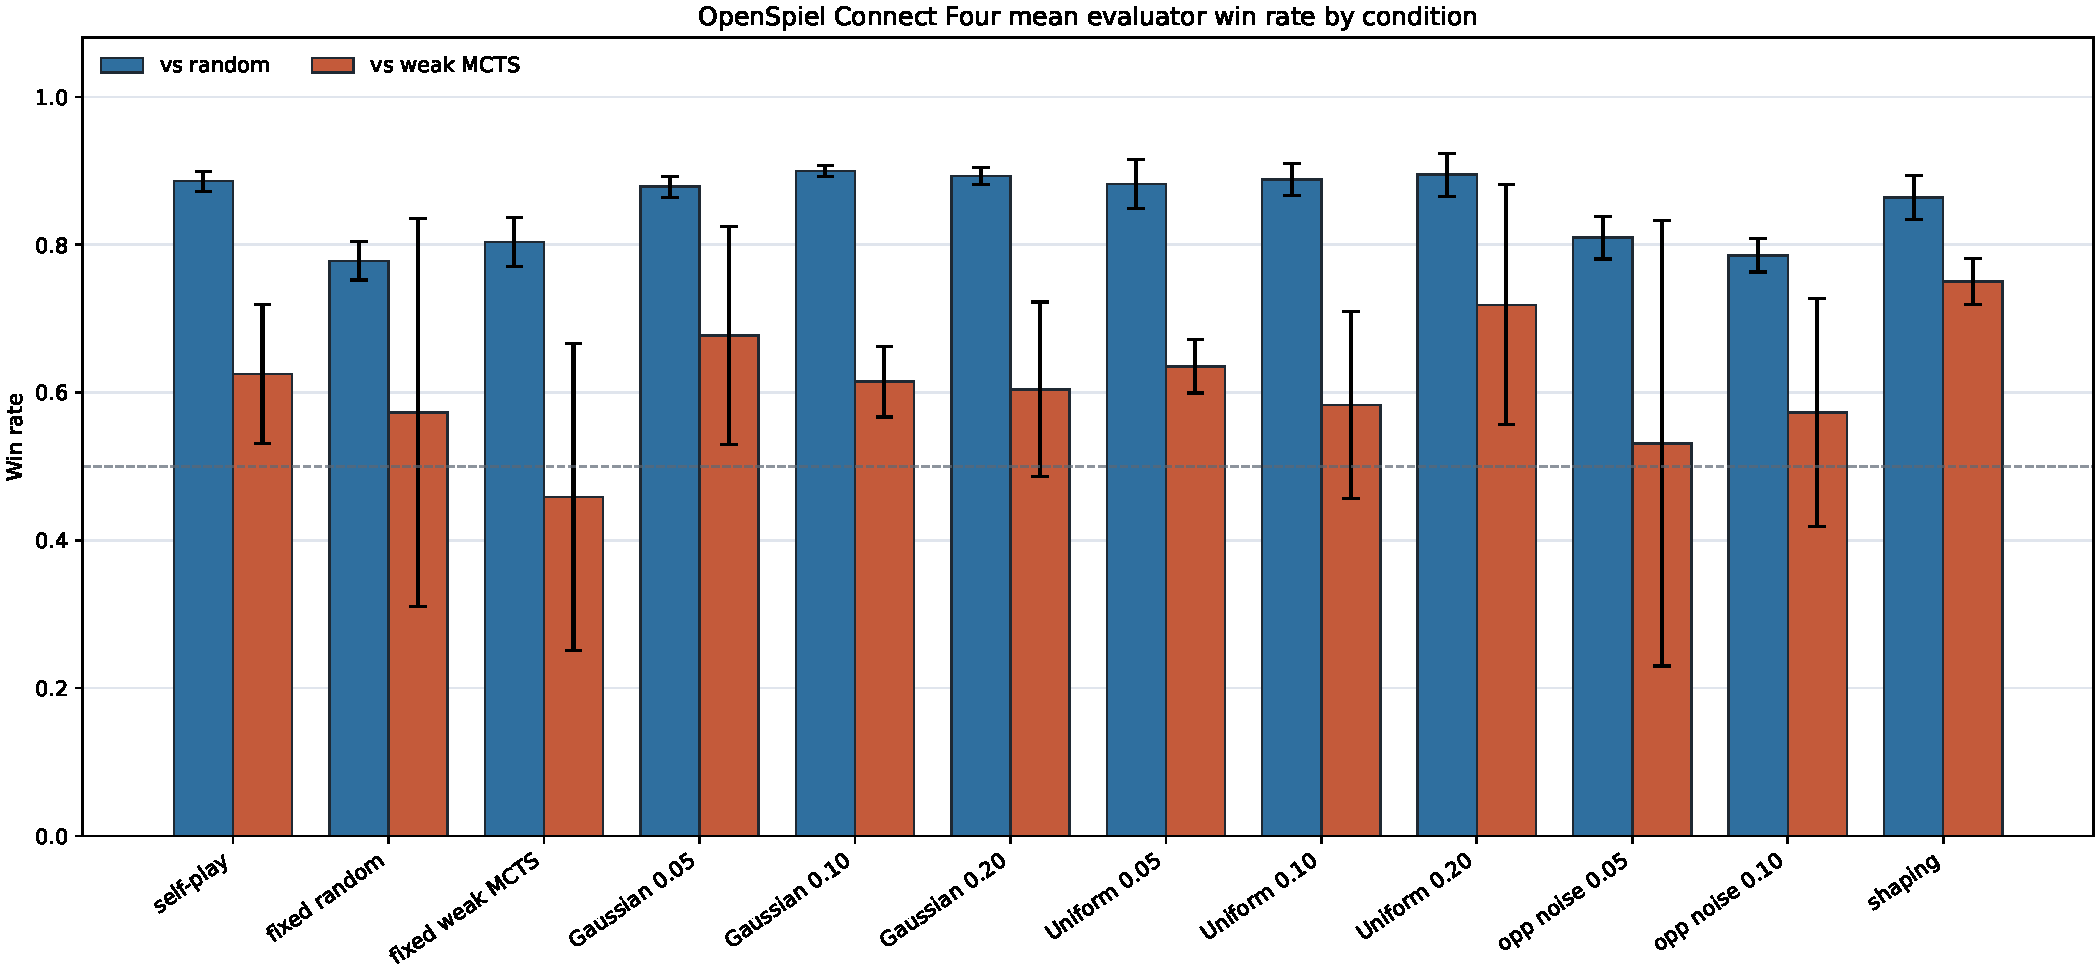
\includegraphics[width=0.86\linewidth]{figures/openspiel_c4_mean_win_rate_by_condition.pdf}
  \caption{Connect Four evaluation under different training conditions. Self-play renews the opponent and state distribution as the policy changes, whereas fixed or noisy sources can increase update magnitude without necessarily improving external performance.}
  \label{fig:connect-four-self-play}
\end{figure}

The experiments also show why reward variance, outcome entropy, or parameter-update norm should not be identified directly with usable information. Fixed opponents and noisy opponent actions can produce larger gradient norms and parameter updates, but this does not by itself improve external evaluation. Larger updates may reflect distributional instability or target drift rather than stronger learning. Reward-noise results point in the same direction: small or moderate terminal noise can be tolerable in the OpenSpiel setting and may even have a mild regularizing effect, while higher noise in a separate value-fitting experiment clearly degrades learning. Noise variance itself is therefore not information. Only reward variation aligned with policy-controllable differences among trajectories can become an effective training signal.

\subsection{Implications for the RLVR Bottleneck}

AlphaZero-like self-play suggests a useful baseline for thinking about information bottlenecks:
\begin{enumerate}
  \item \textbf{The verifier can be terminal and binary.} The reward channel is still low-bandwidth at the trajectory level.
  \item \textbf{The rollout distribution is adaptive.} Self-play keeps generating trajectories near the current decision boundary.
  \item \textbf{The reward variance need not decay.} Because the opponent is the current policy, the outcome distribution remains close to balanced.
  \item \textbf{The global information integral can keep growing.} With continuing self-play and non-vanishing cumulative update budget, the total reward-information mass is not capped by a fixed dataset.
\end{enumerate}

This explains why AlphaZero-like methods can learn from terminal verifiable rewards despite their local low bandwidth. They do not solve the bottleneck by making each reward more informative; they solve it by making the feedback source renewable and by keeping the model near a high-variance self-play frontier. Fixed-dataset \llm{} \rlvr{} lacks this mechanism by default, which is why its information budget is much more likely to saturate.

\section{Fixed-Dataset LLM RLVR: A Non-Renewable Verifier Source}

We now turn to \llm{} \rlvr{} on a fixed prompt dataset. This is the regime where the information bottleneck is sharpest. The verifier can be nearly unbiased: a mathematical answer is correct or incorrect, a program passes or fails tests, and a formal proof is accepted or rejected by a checker. Yet the source of verifier feedback is not renewable in the AlphaZero-like sense. The prompt set and its verifiers are fixed before training, and training only changes which rollouts are sampled from this fixed source.

\subsection{Prompt-Level Bernoulli Feedback}

Let the dataset be
\[
  \mathcal{D}=\{x_i\}_{i=1}^N,
\]
where each prompt $x_i$ has a deterministic binary verifier
\[
  V_i(\tau)\in\{0,1\}.
\]
At training time $t$, the model samples a response trajectory
\[
  \tau\sim q_{\theta(t)}(\cdot\mid x_i),
\]
and the verifier success probability is
\[
  p_i(t)
  =
  \Pr_{\tau\sim q_{\theta(t)}(\cdot\mid x_i)}
  [V_i(\tau)=1].
\]
The local reward variance is therefore
\[
  \mathcal{V}_i(t)
  =
  \Var_{\tau\sim q_{\theta(t)}(\cdot\mid x_i)}
  [V_i(\tau)]
  =
  p_i(t)(1-p_i(t)).
\]
This is maximized only when $p_i(t)=1/2$. If the model always fails a prompt, $p_i(t)\approx 0$ and the verifier gives no local contrast. If the model always solves a prompt, $p_i(t)\approx 1$ and the verifier again gives no local contrast. Thus a fixed prompt contributes useful binary verifier information only while it sits near the current model's decision boundary.

The contrast with self-play is immediate. In AlphaZero-like self-play, the task distribution moves with the learner, so the outcome can remain close to half win and half loss. In fixed-dataset \llm{} \rlvr{}, the prompts do not automatically move. As the model improves, many prompts leave the high-variance region and become all-correct; prompts that are too hard may remain all-wrong. The effective learning signal concentrates on the subset of prompts with intermediate success probability.

\subsection{Group-Relative Updates and Zero-Variance Groups}

Most \llm{} \rlvr{} pipelines do not observe the full Bernoulli distribution for a prompt. They sample a finite group of $K$ rollouts:
\[
  \tau_{i,1},\ldots,\tau_{i,K}
  \sim
  q_{\theta(t)}(\cdot\mid x_i),
  \qquad
  r_{i,j}=V_i(\tau_{i,j}).
\]
The group-centered reward variance is
\[
  \widehat{\mathcal{V}}_{i,K}(t)
  =
  \frac{1}{K}
  \sum_{j=1}^K
  (r_{i,j}-\bar r_i)^2.
\]
For Bernoulli verifier rewards,
\[
  \E[\widehat{\mathcal{V}}_{i,K}(t)]
  =
  \frac{K-1}{K}
  p_i(t)(1-p_i(t)).
\]
A group-relative method such as GRPO receives a nontrivial advantage signal only when the sampled group contains both successes and failures. The probability of this mixed-reward event is
\[
  P_{\mathrm{mixed}}(i,t)
  =
  1-p_i(t)^K-(1-p_i(t))^K.
\]
When $p_i(t)$ is close to $0$ or $1$, the group is very likely to be all-zero or all-one, and the centered verifier signal vanishes. This gives a concrete operational meaning to the bottleneck: a prompt can still be meaningful, and its verifier can still be unbiased, while the sampled group provides no policy-gradient contrast.

\subsection{The Fixed Source Budget}

For a finite training run with update steps $n=1,\ldots,S$, learning rates $\alpha_n$, prompt sampling weights $a_{i,n}$, and $K_{i,n}$ rollouts per selected prompt, the realized empirical verifier-information mass is
\[
  \widehat{\mathcal{I}}_{\llm}
  =
  \sum_{n=1}^{S}
  \alpha_n
  \sum_{i=1}^{N}
  a_{i,n}
  \widehat{\mathcal{V}}_{i,K_{i,n}}(n).
\]
Because verifier rewards are binary,
\[
  \widehat{\mathcal{V}}_{i,K_{i,n}}(n)\le \frac{1}{4},
\]
and therefore
\[
  \widehat{\mathcal{I}}_{\llm}
  \le
  \frac{1}{4}
  \sum_{n=1}^{S}
  \alpha_n
  \sum_{i=1}^{N}
  a_{i,n}.
\]
If each step samples from a normalized prompt distribution, $\sum_i a_{i,n}=1$, then
\[
  \widehat{\mathcal{I}}_{\llm}
  \le
  \frac{1}{4}
  \sum_{n=1}^{S}\alpha_n.
\]
If one counts the unnormalized dataset total, the corresponding bound is
\[
  \widehat{\mathcal{I}}_{\mathcal{D}}^{\mathrm{tot}}
  \le
  \frac{N}{4}
  \sum_{n=1}^{S}\alpha_n.
\]
Thus, for a fixed dataset, fixed verifier family, fixed rollout budget, and fixed update schedule, the maximum binary verifier-information mass is fixed before training begins. The algorithm can change how much of this ceiling is actually realized, but it cannot make the source itself renewable. This is the sense in which \llm{} \rlvr{} has a fixed verifier-information budget on a given dataset.

\begin{discussionbox}[title={Discussion: Fixed does not mean fully used}]
The fixed-source statement is not that every algorithm extracts the same amount of useful information. Most algorithms extract only a fraction of the available verifier-information mass. Some waste rollouts on already-solved prompts, some sample near-identical trajectories, and some allocate updates to verifier variance that is poorly aligned with useful reasoning changes. The point is that, unlike self-play, the dataset-verifier source does not automatically create new high-variance tasks as the model improves. Improvements must come from better allocation, better exploration, denser feedback, or adding new data.
\end{discussionbox}

\subsection{Why the Signal Saturates}

The prompt-level picture suggests a simple phase diagram:
\[
  p_i(t)\approx 0
  \quad\Rightarrow\quad
  \text{all failures, no contrast},
\]
\[
  p_i(t)\approx \frac{1}{2}
  \quad\Rightarrow\quad
  \text{mixed outcomes, strong contrast},
\]
\[
  p_i(t)\approx 1
  \quad\Rightarrow\quad
  \text{all successes, no contrast}.
\]
Training is most efficient when many prompts lie in the middle regime. However, a fixed dataset does not keep prompts there. As competence increases, easy prompts move into the all-success region. If the remaining prompts are too hard, they may stay in the all-failure region. The total effective verifier signal can therefore peak early and then decay, even though the verifier remains correct.

This view also clarifies why several recent \rlvr{} interventions are useful. Rollout-diversification methods try to increase the chance that a group contains genuinely different trajectories, raising $P_{\mathrm{mixed}}$ near the decision boundary \cite{lookahead_rollouts_2026,eepo_2026}. Entropy or advantage-shaping methods try to prevent useful prompts from being discarded merely because their sampled group has zero variance \cite{exploration_exploitation_rlvr_2026,no_prompt_left_behind_2026}. Hybrid reward methods add dense or graded feedback so that rollouts can differ even when the terminal verifier is identical \cite{hybrid_reinforcement_2026}. In the language of this paper, these methods do not primarily make the verifier less biased; they increase the effective bandwidth between the fixed verifier source and the optimizer.

\subsection{Algorithmic Consequences}

Fixed-dataset \llm{} \rlvr{} should therefore be evaluated by how efficiently it uses its verifier source. The most direct quantities are:
\begin{enumerate}
  \item \textbf{Exposed verifier variance.} How much of $\sum_i p_i(t)(1-p_i(t))$ is actually sampled under the rollout budget?
  \item \textbf{Mixed-group rate.} What fraction of prompt groups contain both successes and failures?
  \item \textbf{Update conversion.} How much covariance between verifier rewards and rollout scores survives clipping, KL regularization, and reward normalization?
  \item \textbf{Prompt allocation.} Are updates spent on prompts near the decision boundary, or wasted on all-correct and all-wrong groups?
  \item \textbf{Dataset refresh.} Does the system introduce new prompts, harder variants, self-generated tasks, or curriculum mechanisms that renew the high-variance frontier?
\end{enumerate}

The central contrast is now clear. AlphaZero-like self-play can keep a binary terminal reward useful because the environment distribution is adaptive and self-renewing. Fixed-dataset \llm{} \rlvr{} starts from a fixed collection of verifier-defined objectives. Its core problem is not only sparse credit assignment, but also the depletion and misallocation of a finite verifier-information source.

\section{Single-Question LLM RLVR Dynamics}

The previous section described fixed-dataset \llm{} \rlvr{} as a non-renewable verifier source. The atomic unit of that source is a single question or prompt. We therefore first give the one-question case its own compact empirical dynamics. This is not meant to be the general theory for all \rlvr{} settings, nor even the full dataset-level theory for \llm{} \rlvr{}. It is a falsifiable base model for a fixed prompt with a binary verifier, especially single-question runs where success rate, action entropy, and cumulative reward-information mass are all observable. The model uses only three observed quantities:
\[
  I_t
  \quad
  A_t
  \quad
  p_t,
\]
where $p_t$ is the rollout success rate, $A_t$ is the average per-token action entropy, and $I_t$ is the cumulative reward-information mass observed up to training step $t$.

This section should be read as the \llm{}-specific bridge between the covariance/variance formulation and single-question experiments. If the model fits observed curves better than reward variance alone, then action entropy is not merely a side diagnostic. It is part of the prompt-level \llm{} bottleneck itself. Dataset-level \llm{} dynamics can then be treated as a mixture of many such one-question systems, with allocation, interference, and task imbalance layered on top. After deriving regime-specific dynamics for self-play, \llm{} \rlvr{}, and diffusion-model \rlvr{}, we can abstract a common theory.

\subsection{Observed State Variables}

For a fixed problem $x$, define
\[
  p_t
  =
  \Pr_{\tau\sim q_{\theta_t}(\cdot\mid x)}
  [V(x,\tau)=1],
\]
estimated by the success rate of rollouts at step $t$. Let
\[
  A_t
  =
  \E_{\tau\sim q_{\theta_t}(\cdot\mid x)}
  \left[
    \frac{1}{|\tau|}
    \sum_{\ell=1}^{|\tau|}
    H\big(\pi_{\theta_t}(\cdot\mid h_\ell)\big)
  \right]
\]
be the average per-token action entropy along sampled rollouts, where $h_\ell$ is the generation history before token $\ell$. Finally, let
\[
  I_t
  =
  \sum_{n<t}
  \alpha_n \widehat{\mathcal{V}}_n(x)
\]
be the cumulative observed information mass, with increment
\[
  \Delta I_t=I_{t+1}-I_t.
\]

Here $\widehat{\mathcal{V}}_n(x)$ is the empirical version of the local reward variance defined in Section~2:
\[
  \mathcal{V}_{\theta_n}(x)
  =
  \Var_{\tau\sim q_{\theta_n}(\cdot\mid x)}
  [V(x,\tau)].
\]
For a binary verifier,
\[
  \mathcal{V}_{\theta_t}(x)
  =
  p_t(1-p_t).
\]
We will use the normalized reward variance
\[
  \overline{\mathcal{V}}_t(x)
  =
  4\mathcal{V}_{\theta_t}(x)
  =
  4p_t(1-p_t)
  \in[0,1].
\]
This differs from the raw Bernoulli variance only by a constant factor. The normalization is convenient because $\overline{\mathcal{V}}_t(x)=1$ at the maximally mixed success rate $p_t=1/2$. Thus $p_t$ is not a replacement for the paper's variance notation; it is the binary-verifier parameterization of $\mathcal{V}_{\theta_t}(x)$.

\subsection{A Two-Sided Action-Entropy Bottleneck}

Action entropy affects learning in two opposite ways. If $A_t$ is too small, the model does not explore enough distinct rollouts and the verifier sees little contrast. If $A_t$ is too large, credit assignment becomes diluted across a large action space: even when the verifier observes success and failure, the update may be spread over too many weakly identified token choices.

We model this trade-off with a two-sided bottleneck function
\[
  B(A_t)
  =
  \left(1-\exp\left(-\frac{A_t}{A_{\mathrm{exp}}}\right)\right)
  \exp\left(-\frac{A_t}{A_{\mathrm{credit}}}\right).
\]
The first factor is an exploration gate. It is small when action entropy is too low. The second factor is a credit-assignment penalty. It is small when action entropy is too high. Therefore $B(A)$ is inverted-U shaped.

The entropy level that maximizes this bottleneck is
\[
  A^\star
  =
  A_{\mathrm{exp}}
  \log\left(1+\frac{A_{\mathrm{credit}}}{A_{\mathrm{exp}}}\right).
\]
This gives a concrete prediction: useful verifier-information extraction should concentrate near an intermediate action entropy, rather than increasing monotonically with entropy.

\subsection{Three-Variable Dynamics}

We propose the following closed dynamical system:
\[
  \Delta I_t
  =
  \kappa\,
  \overline{\mathcal{V}}_t(x)\,
  B(A_t)\,
  \left(1-\frac{I_t}{I_\infty}\right)_+,
\]
\[
  \Delta \logit(p_t)
  =
  \eta
  \frac{\Delta I_t}{(A_t+\epsilon)^\rho},
\]
\[
  \Delta A_t
  =
  -\beta\,\Delta I_t\,A_t
  +
  \xi\,\overline{\mathcal{V}}_t(x)(A_{\mathrm{mix}}-A_t),
\]
where $(u)_+=\max(u,0)$. The positive-part operator is a modeling safeguard: once the fitted cumulative information reaches the problem-specific ceiling $I_\infty$, the remaining-information term should not become negative.

The parameters have the following interpretation:
\begin{center}
\begin{tabular}{ll}
\toprule
Parameter & Meaning \\
\midrule
$\kappa$ & information extraction rate \\
$I_\infty$ & total learnable information for this problem \\
$\eta$ & conversion rate from extracted information to success \\
$\rho$ & credit concentration exponent \\
$\beta$ & entropy-collapse rate caused by learning \\
$\xi$ & entropy re-mixing strength in mixed success/failure regimes \\
$A_{\mathrm{exp}}$ & entropy scale needed for exploration \\
$A_{\mathrm{credit}}$ & entropy scale where credit assignment becomes diluted \\
$A_{\mathrm{mix}}$ & mixed or exploratory entropy attractor \\
$\epsilon$ & numerical stabilizer \\
\bottomrule
\end{tabular}
\end{center}

\paragraph{Information increment.}
The first equation says that information extraction requires three simultaneous conditions:
\[
  \overline{\mathcal{V}}_t(x)>0,\qquad B(A_t)>0,\qquad I_t<I_\infty.
\]
The model predicts
\[
  \Delta I_t\to 0
  \quad\text{when}\quad
  p_t\to 0,\; p_t\to 1,\; A_t\to 0,\; A_t\to\infty,\; \text{or}\; I_t\to I_\infty.
\]
Thus a verifier can be unbiased and still produce little information if the policy is always wrong, always correct, too deterministic, too diffuse, or has already exhausted the learnable information for that problem.

\paragraph{Success-rate improvement.}
The second equation links extracted information to success:
\[
  \Delta \logit(p_t)
  =
  \eta
  \frac{\Delta I_t}{(A_t+\epsilon)^\rho}.
\]
The logit scale is used because it separates additive progress from probability saturation near $0$ and $1$. For fitting, $p_t$ should be clipped to $[\epsilon_p,1-\epsilon_p]$ before taking logits. The denominator captures credit concentration: given the same $\Delta I_t$, lower action entropy can produce a larger success-rate gain because probability mass is concentrated on fewer actions. This does not mean lower entropy is always better, because the first equation already makes $\Delta I_t$ small when $A_t$ is too low.

\paragraph{Action-entropy dynamics.}
The third equation contains two forces:
\[
  -\beta\,\Delta I_t\,A_t
\]
models entropy collapse caused by decisive learning, while
\[
  \xi\,\overline{\mathcal{V}}_t(x)(A_{\mathrm{mix}}-A_t)
\]
models re-mixing when the model is in a mixed success/failure regime. This allows non-monotone entropy curves: entropy can decrease during decisive learning, temporarily increase near a difficult boundary, and flatten after the problem is solved or fully failed.

\begin{discussionbox}[title={Discussion: Why include action entropy?}]
The fixed-dataset theory in the previous section would suggest that $\mathcal{V}_{\theta_t}(x)$ is the main local source of verifier information for one prompt. The three-variable model tests whether this is sufficient in single-question \llm{} training. If $\Delta I_t$ is better explained by $\overline{\mathcal{V}}_t(x)B(A_t)$ than by $\overline{\mathcal{V}}_t(x)$ alone, then action entropy is not just a proxy for exploration. It is a measurable bottleneck that controls how much verifier information can be exposed and converted into updates.
\end{discussionbox}

\subsection{Reduced Model for First Experiments}

The full three-equation system may be too flexible for a first pass. A simpler first test keeps only the information and success equations:
\[
  \Delta I_t
  =
  \kappa\,
  \overline{\mathcal{V}}_t(x)\,
  B(A_t)\,
  \left(1-\frac{I_t}{I_\infty}\right)_+,
\]
\[
  \Delta \logit(p_t)
  =
  \eta
  \frac{\Delta I_t}{(A_t+\epsilon)^\rho}.
\]
The entropy curve can then be fit separately by
\[
  A_{t+1}
  =
  A_t-\beta\,\Delta I_t\,A_t,
\]
or equivalently,
\[
  \Delta \log A_t
  \approx
  -\beta\,\Delta I_t
\]
during decisive learning phases. This reduced form is likely the most robust first empirical test because it avoids over-attributing short-term entropy fluctuations to the re-mixing term.

\subsection{Empirical Tests}

The model gives several direct tests on single-question curves.

\paragraph{Test 1: inverted-U action bottleneck.}
Compute
\[
  Y_t=\frac{\Delta I_t}{\overline{\mathcal{V}}_t(x)+\epsilon_v}.
\]
If the bottleneck hypothesis is correct, $Y_t$ should be low when $A_t$ is very small, high at intermediate $A_t$, and lower again when $A_t$ is very large. A monotone relationship would argue against the proposed two-sided bottleneck.

\paragraph{Test 2: information-to-success conversion.}
Fit
\[
  \Delta \logit(p_t)
  =
  \eta
  \frac{\Delta I_t}{(A_t+\epsilon)^\rho}.
\]
Equivalently,
\[
  \frac{\Delta \logit(p_t)}{\Delta I_t+\epsilon_I}
  \propto
  (A_t+\epsilon)^{-\rho}.
\]
The prediction is that, conditional on the same extracted information, lower action entropy yields larger success-rate gain.

\paragraph{Test 3: entropy collapse with information.}
Fit
\[
  \Delta A_t
  =
  -\beta\,\Delta I_t\,A_t
\]
or
\[
  \Delta \log A_t
  =
  -\beta\,\Delta I_t.
\]
The prediction is that $\log A_t$ should be approximately linear in $I_t$ during decisive learning phases.

\paragraph{Test 4: finite information ceiling.}
The first equation predicts that
\[
  I_t\to I_\infty
\]
when the problem is learnable and reaches a solved regime. Thus $\Delta I_t$ should decay as $I_t$ approaches a problem-specific ceiling. However, if a problem remains in a persistent mixed regime, with $p_t$ away from $0$ and $1$ and $A_t$ near $A^\star$, then $\Delta I_t$ may remain positive for a long time. Such cases are especially valuable because they test whether the finite-information assumption is wrong, or whether the fitted $I_\infty$ is much larger than the observed training horizon.

\subsection{Practical Fitting Protocol}

For each completed single-question run, we can fit the model as follows:
\begin{enumerate}
  \item Smooth $p_t$, $A_t$, and $I_t$ lightly if the curves are noisy.
  \item Compute $\Delta I_t=I_{t+1}-I_t$, $\Delta z_t=\logit(p_{t+1})-\logit(p_t)$, and $\overline{\mathcal{V}}_t=4p_t(1-p_t)$.
  \item Fit the information equation
  \[
    \Delta I_t
    \sim
    \overline{\mathcal{V}}_t B(A_t)\left(1-\frac{I_t}{I_\infty}\right)_+.
  \]
  \item Fit the success equation
  \[
    \Delta z_t
    \sim
    \frac{\Delta I_t}{(A_t+\epsilon)^\rho}.
  \]
  \item Fit the entropy equation
  \[
    \Delta A_t
    \sim
    -\Delta I_t A_t + \overline{\mathcal{V}}_t(A_{\mathrm{mix}}-A_t).
  \]
\end{enumerate}

The key empirical comparison is between the one-factor model
\[
  \Delta I_t\sim \overline{\mathcal{V}}_t(x)
\]
and the full bottleneck model
\[
  \Delta I_t
  \sim
  \overline{\mathcal{V}}_t(x)B(A_t)\left(1-\frac{I_t}{I_\infty}\right)_+.
\]
If the full model gives a significantly better fit, then the one-question bottleneck is not only a property of success variance. It also depends on action entropy and remaining learnable information.

\subsection{Reading Three-Line Curves}

The model suggests the following interpretation of the three observed curves:
\begin{center}
\begin{tabular}{p{0.19\linewidth}p{0.36\linewidth}p{0.34\linewidth}}
\toprule
Regime & Curve pattern & Interpretation \\
\midrule
Dead exploration & $p_t$ near $0$, $I_t$ flat, $A_t$ high & No reward signal is converted. \\
Effective learning & $p_t$ rising, $I_t$ rising, $A_t$ falling & Information extraction with entropy collapse. \\
Solved state & $p_t$ near $1$, $I_t$ flat, $A_t$ low & Verifier information is exhausted. \\
Mixed boundary & $p_t$ unstable, $I_t$ rising, $A_t$ non-monotone & Useful test of finite ceiling. \\
\bottomrule
\end{tabular}
\end{center}

This gives a compact experimental agenda. The simplest hypothesis is that verifier information is controlled only by success variance. The stronger bottleneck hypothesis is that success variance, action entropy, and remaining cumulative information form a coupled system. The difference is measurable from the curves themselves.

\section{Diffusion-Model RLVR}

% TODO: Add theory and experiments for diffusion-model RLVR.


\bibliographystyle{plain}
\bibliography{references}

\end{document}
